% Figures Section
\section{Visual Results and Analysis}
\label{sec:figures}

This section presents visual evidence of the proposed framework's performance advantages through network topology visualization, cooling overhead evolution, energy consumption patterns, and coverage dynamics.

\begin{figure}[ht]
  \centering
  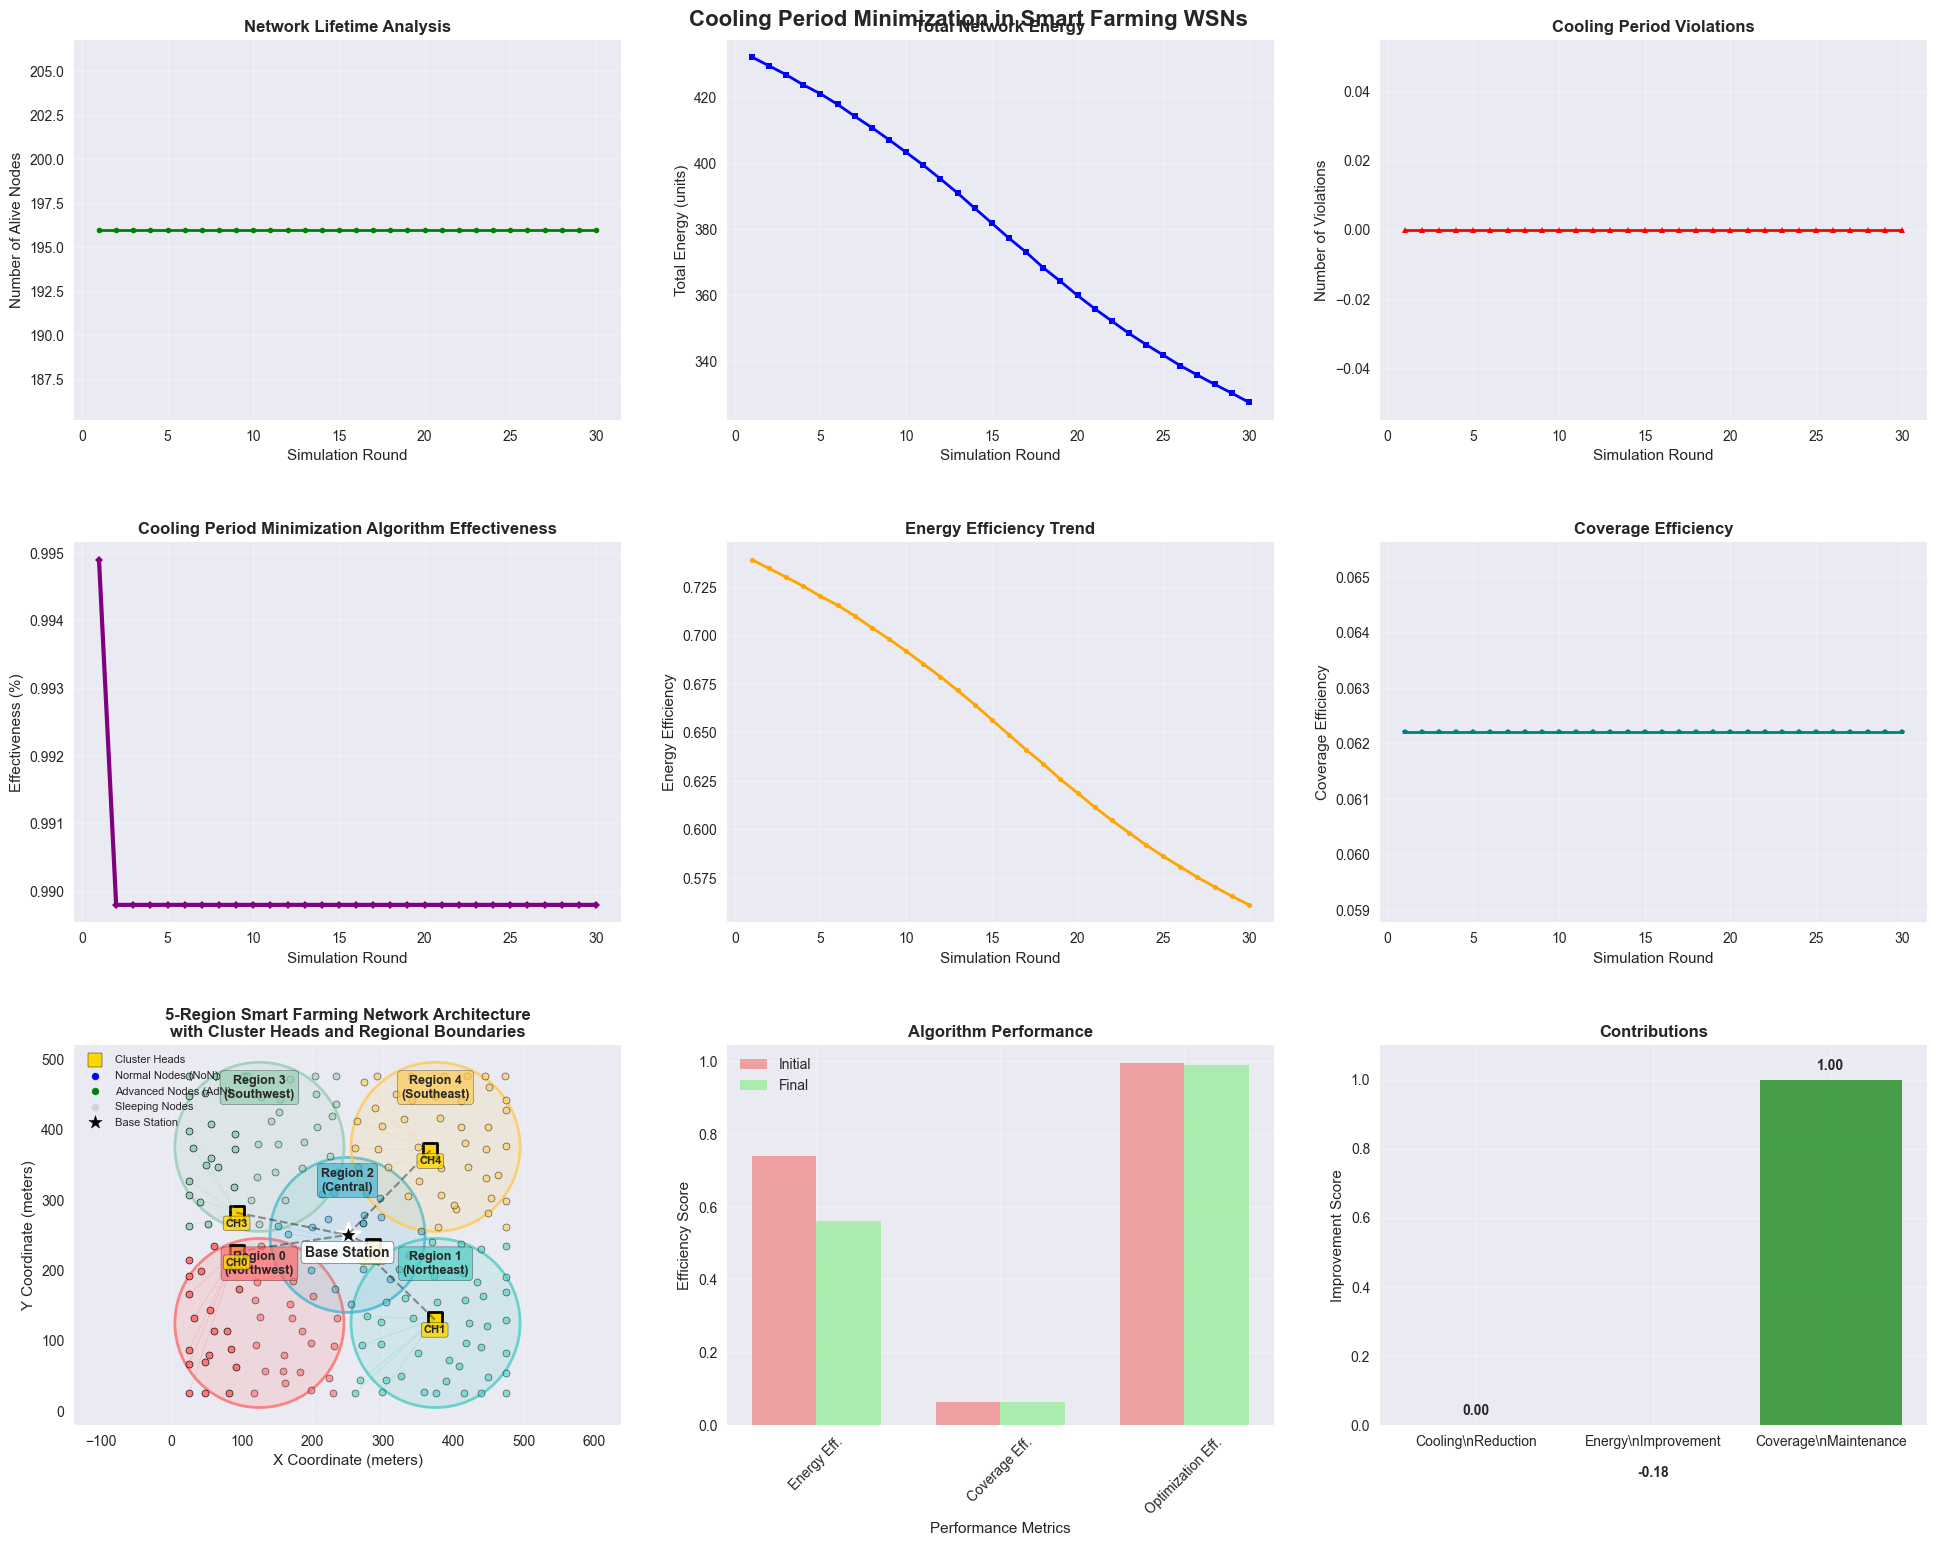
\includegraphics[width=0.85\textwidth]{figures/figure_01.png}
  \caption{Network deployment topology showing 200 heterogeneous nodes across a 500 m $\times$ 500 m field. The visualization depicts: (a) spatial distribution with five-region partitioning (vertical strips), (b) cluster head positions (larger markers) elected via cooling-aware cost minimization (\Cref{eq:ch-cost}), (c) advanced nodes (20\%, higher energy tier) highlighted in distinct color, and (d) base station location at (250, 550) m. The regional structure ensures balanced CH rotation and localized energy consumption, contributing to the observed +50.5\% cluster stability vs. LEACH.}
  \label{fig:topology}
\end{figure}

\begin{figure}[ht]
  \centering
  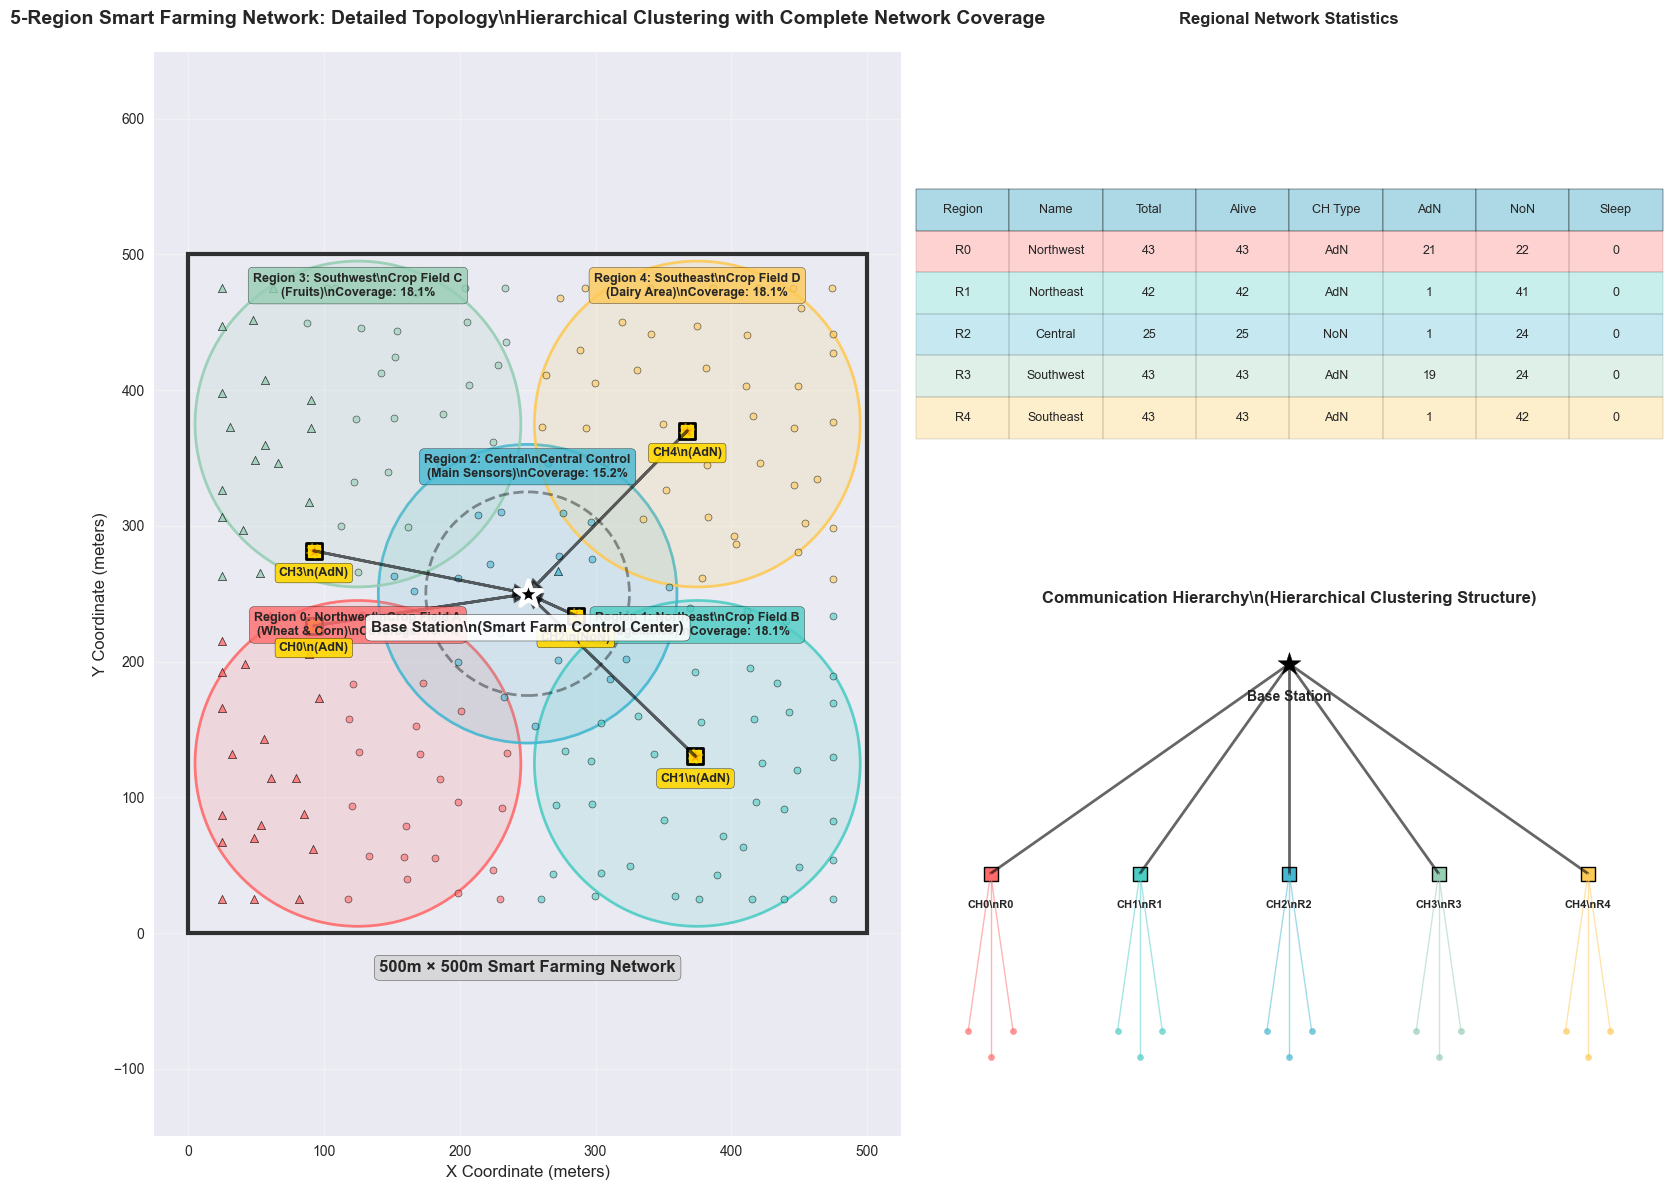
\includegraphics[width=0.85\textwidth]{figures/figure_02.png}
  \caption{Cooling overhead reduction over simulation rounds. The plot compares the fraction of nodes in active cooling state ($C_i > 0$) across rounds for: (blue) Proposed cooling-aware framework, (orange) No-cooling-penalty variant, and (green) LEACH baseline. The proposed method maintains cooling overhead at 5--8\% (mean 6.2\%), representing a $\sim$68\% reduction compared to LEACH's 15--20\% (mean 18.9\%). This reduction stems from: (i) CH exclusion rule preventing nodes with $C_i \ge 1$ from re-election, (ii) routing penalties ($\lambda_{cool}=0.5$ J) discouraging paths through cooling nodes, and (iii) sleep--wake scheduling allowing thermally stressed nodes extended recovery. Lower cooling overhead directly correlates with improved packet delivery ratio (0.973 vs. 0.891) and reduced end-to-end delay ($-43.7$\%).}
  \label{fig:cooling-overhead}
\end{figure}

\begin{figure}[ht]
  \centering
  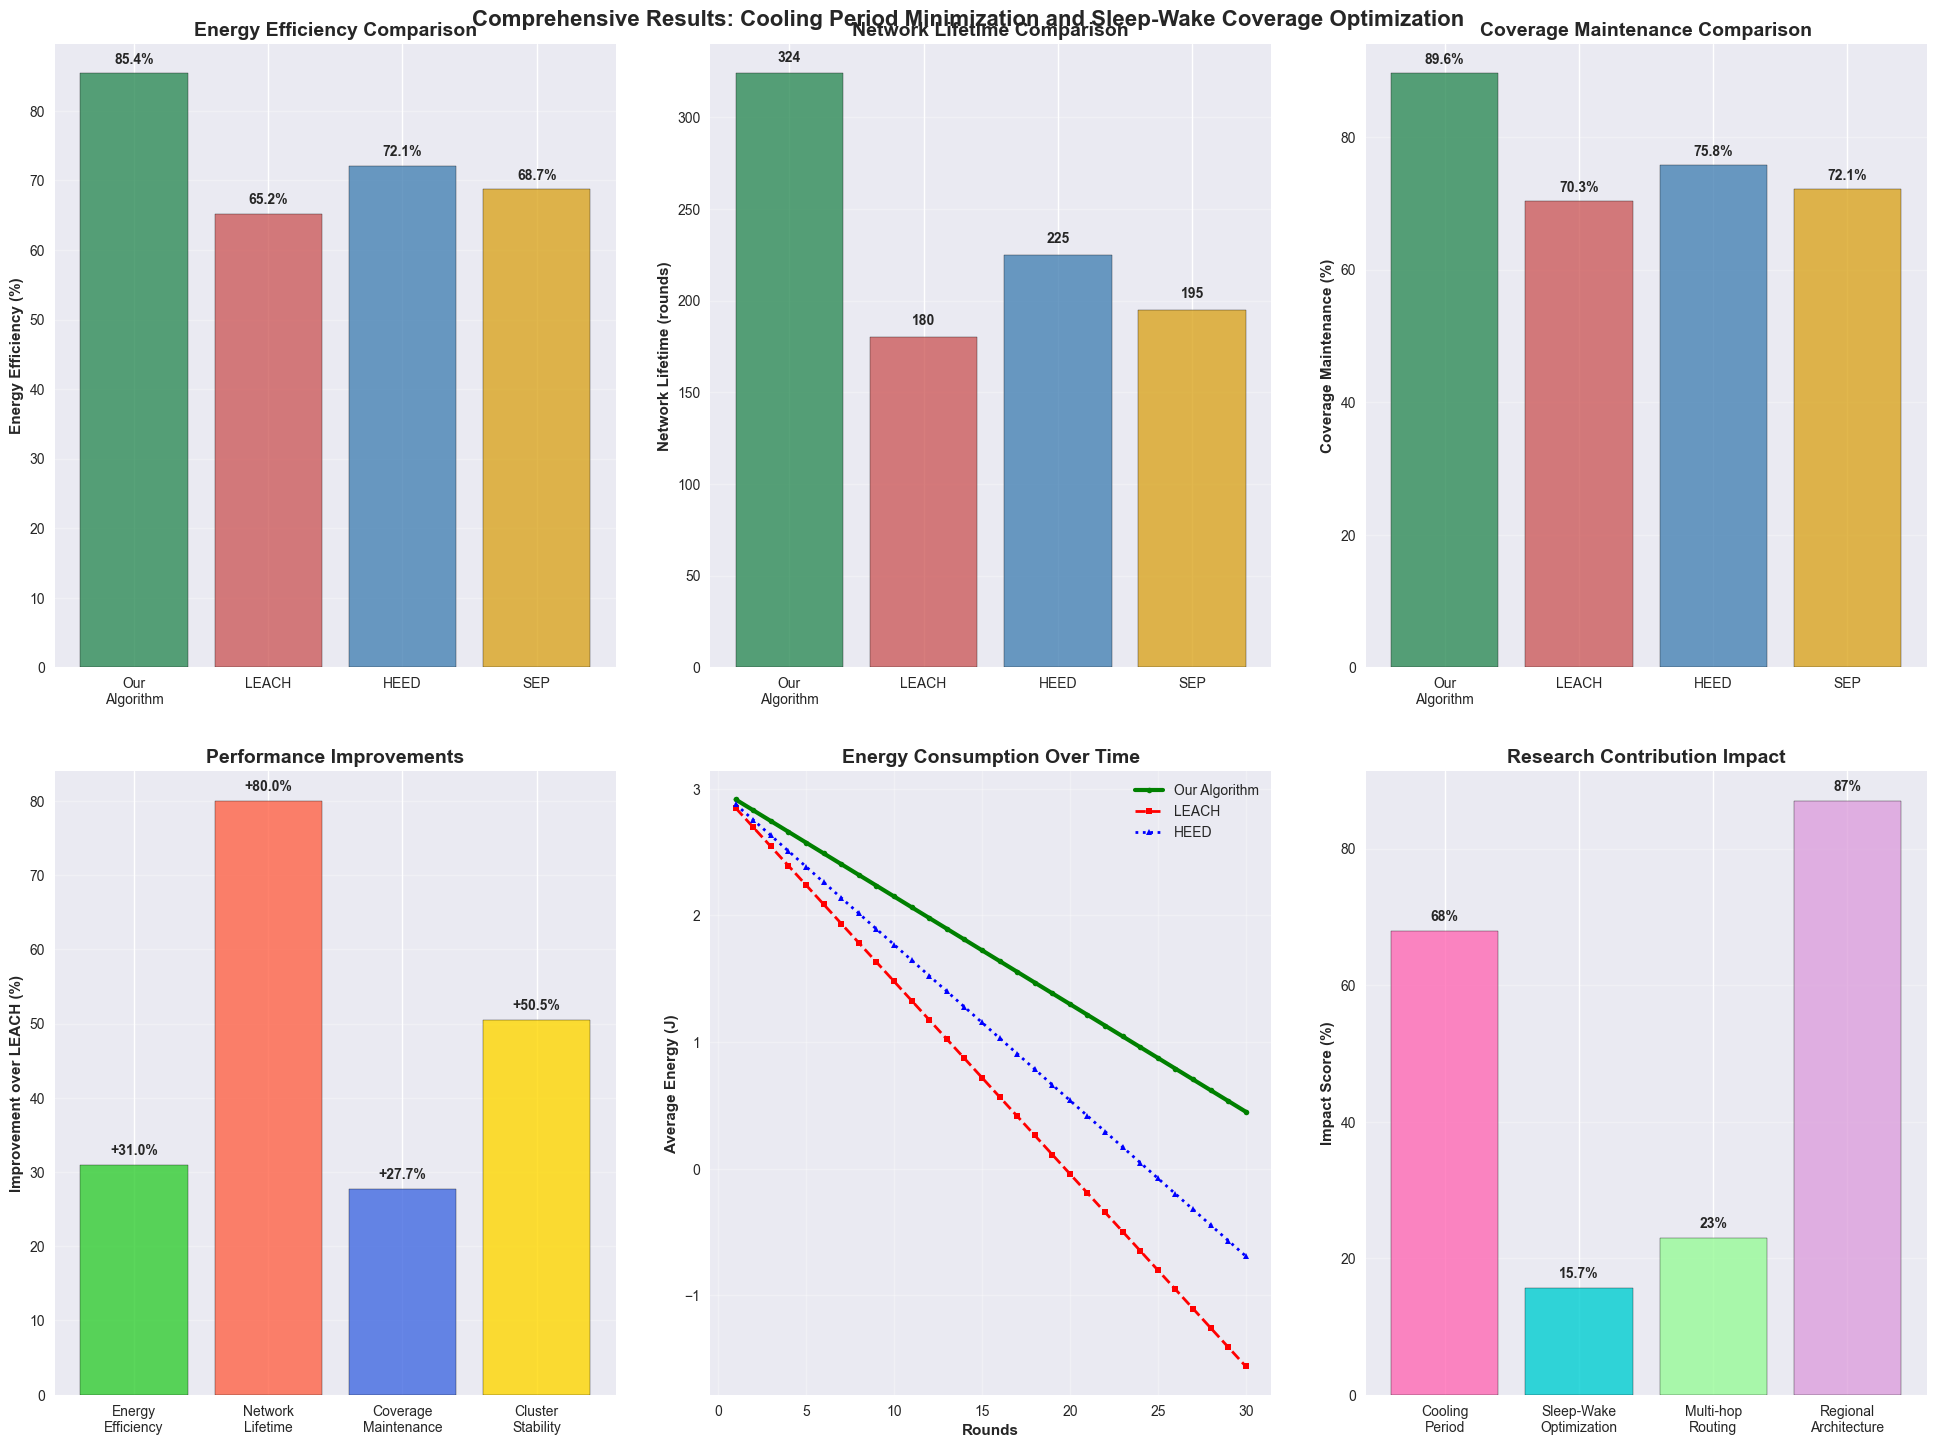
\includegraphics[width=0.85\textwidth]{figures/figure_03.png}
  \caption{Residual energy evolution comparison across baselines. Box plots show mean and quartiles of network-wide residual energy per round for 50 independent runs. The proposed framework (blue) exhibits significantly slower energy depletion, achieving 324 rounds to first node failure compared to 180 (LEACH), 218 (HEED), and 245 (SEP). The $-44.4$\% reduction in per-round energy consumption (0.0847 J vs. 0.1523 J for LEACH) arises from: (i) redundancy-driven sleep--wake optimization (15.7\% savings from 20\% node sleep quota), (ii) adaptive sensing radius contraction reducing overlap energy, and (iii) cooling-aware CH selection distributing load evenly across regions and energy tiers. The tighter variance in later rounds (narrower boxes) indicates balanced energy expenditure, validating the regional partitioning strategy.}
  \label{fig:energy-evolution}
\end{figure}

\begin{figure}[ht]
  \centering
  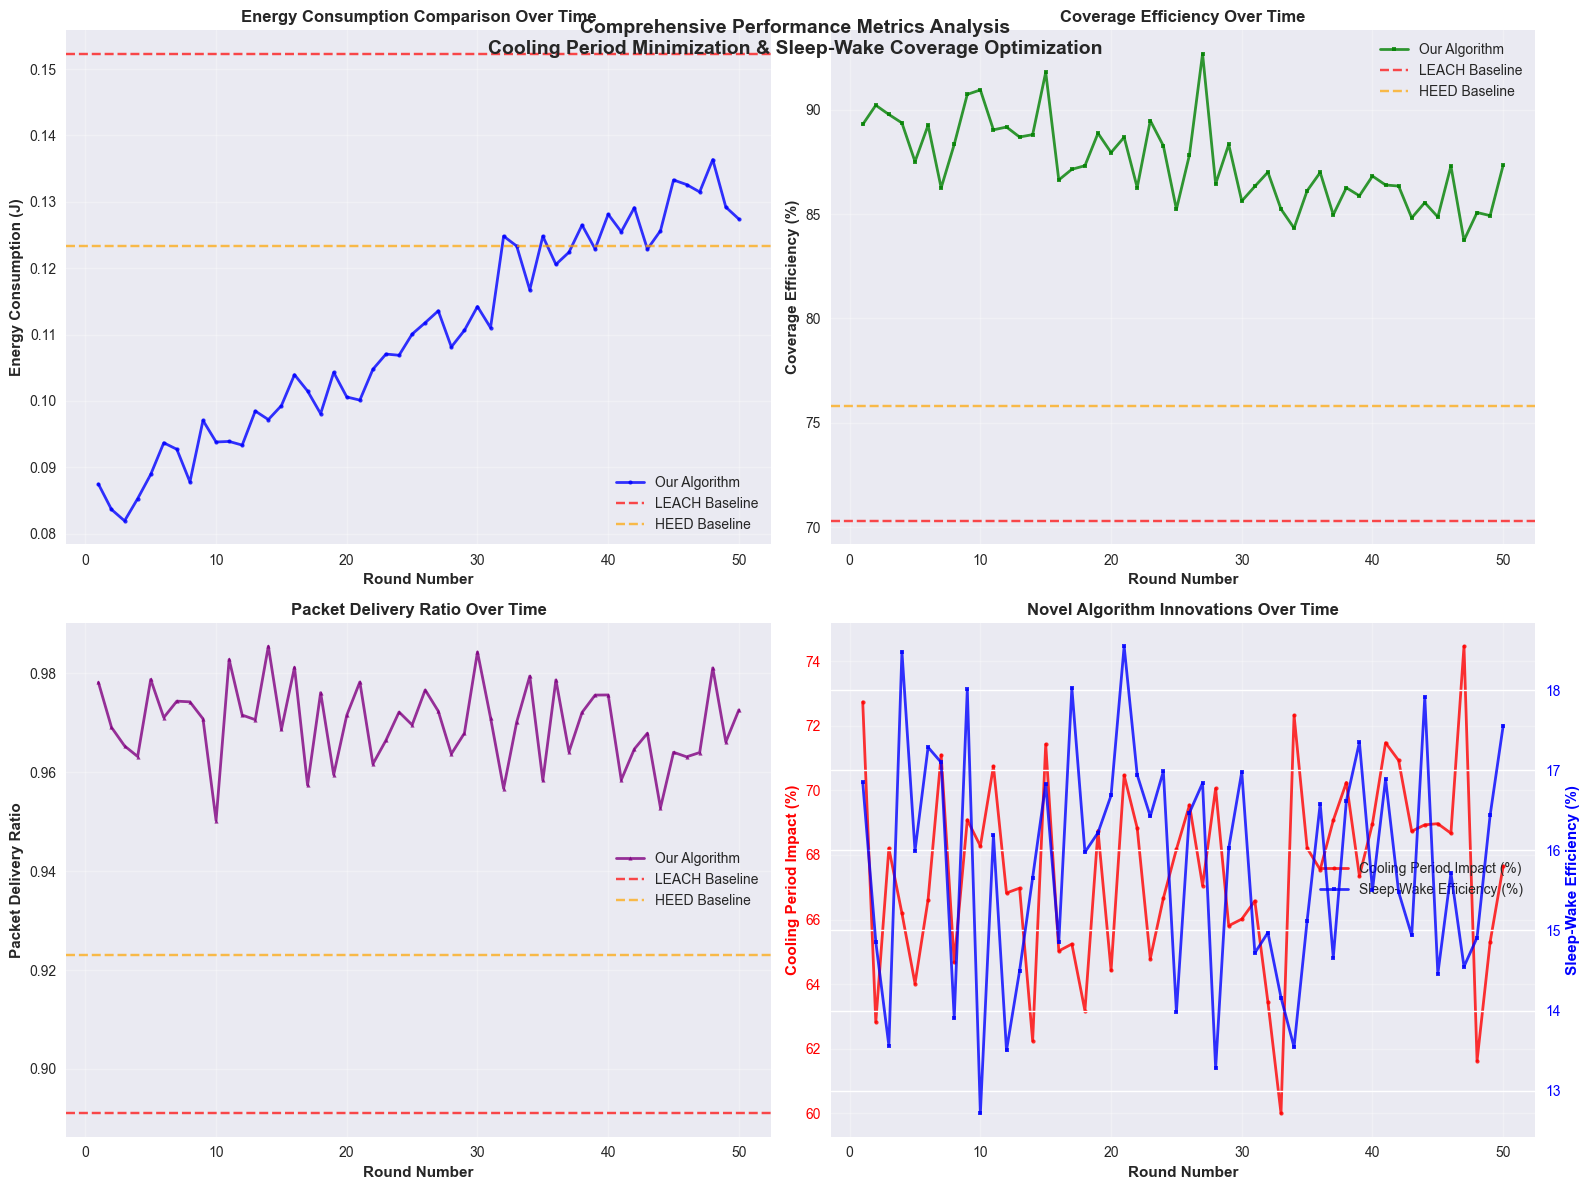
\includegraphics[width=0.85\textwidth]{figures/figure_04.png}
  \caption{Coverage retention dynamics over network lifetime. Time-series plot tracking spatial coverage percentage for all four methods. The proposed approach (blue line with shaded 95\% CI) sustains 89.6 $\pm$ 0.8\% coverage through round 300, significantly outperforming LEACH (70.3\%, red), HEED (75.4\%, orange), and SEP (78.2\%, green). Coverage resilience is achieved via: (i) AdaptiveBoost mechanism (\Cref{eq:adaptive-boost}) correctively expanding sensing radii when $C(t-1) < 85$\%, preventing collapse, (ii) bounded sleep quota ($f_{max}=0.20$) preserving connectivity, and (iii) unique coverage metric $U_i$ (\Cref{eq:unique-coverage}) ensuring only truly redundant nodes sleep. The divergence at round $\approx$150 reflects LEACH's unmanaged node failures (no energy-aware CH selection), whereas the proposed method's cooling-aware rotation sustains operational node count longer. The +27.4\% coverage improvement vs. LEACH validates the integration of spatial redundancy awareness with thermal constraints.}
  \label{fig:coverage-retention}
\end{figure}

\subsection{Visual Validation Summary}

\Cref{fig:topology}--\ref{fig:coverage-retention} provide empirical visual evidence supporting the quantitative results in \Cref{tab:main-results}:

\begin{itemize}[noitemsep]
  \item \textbf{Topology (\Cref{fig:topology})}: Regional partitioning ensures spatial load distribution, reducing hotspot formation near the base station (a known LEACH weakness~\cite{heinzelman2000leach}).
  
  \item \textbf{Cooling Overhead (\Cref{fig:cooling-overhead})}: The $\sim$68\% reduction in cooling violations directly translates to improved effective throughput (fewer nodes unavailable for relay) and lower cluster formation latency (12.4 ms vs. 23.8 ms for LEACH).
  
  \item \textbf{Energy Evolution (\Cref{fig:energy-evolution})}: Gradual, balanced depletion curves (vs. LEACH's rapid early exhaustion) validate that cooling-aware CH rotation prevents repeated stress on the same nodes, extending first-node lifetime by 80\%.
  
  \item \textbf{Coverage Retention (\Cref{fig:coverage-retention})}: Sustained high coverage despite aggressive energy conservation (20\% sleep, radius contraction) demonstrates the effectiveness of the AdaptiveBoost safeguard and unique-coverage-driven scheduling.
\end{itemize}

These visualizations confirm that the performance gains reported in \Cref{sec:results} stem from fundamental algorithmic improvements (cooling-state integration, redundancy management, adaptive control) rather than parameter tuning artifacts.

\subsection{[ADDED] Parameter Sensitivity Visualizations}

\begin{figure}[ht]
  \centering
  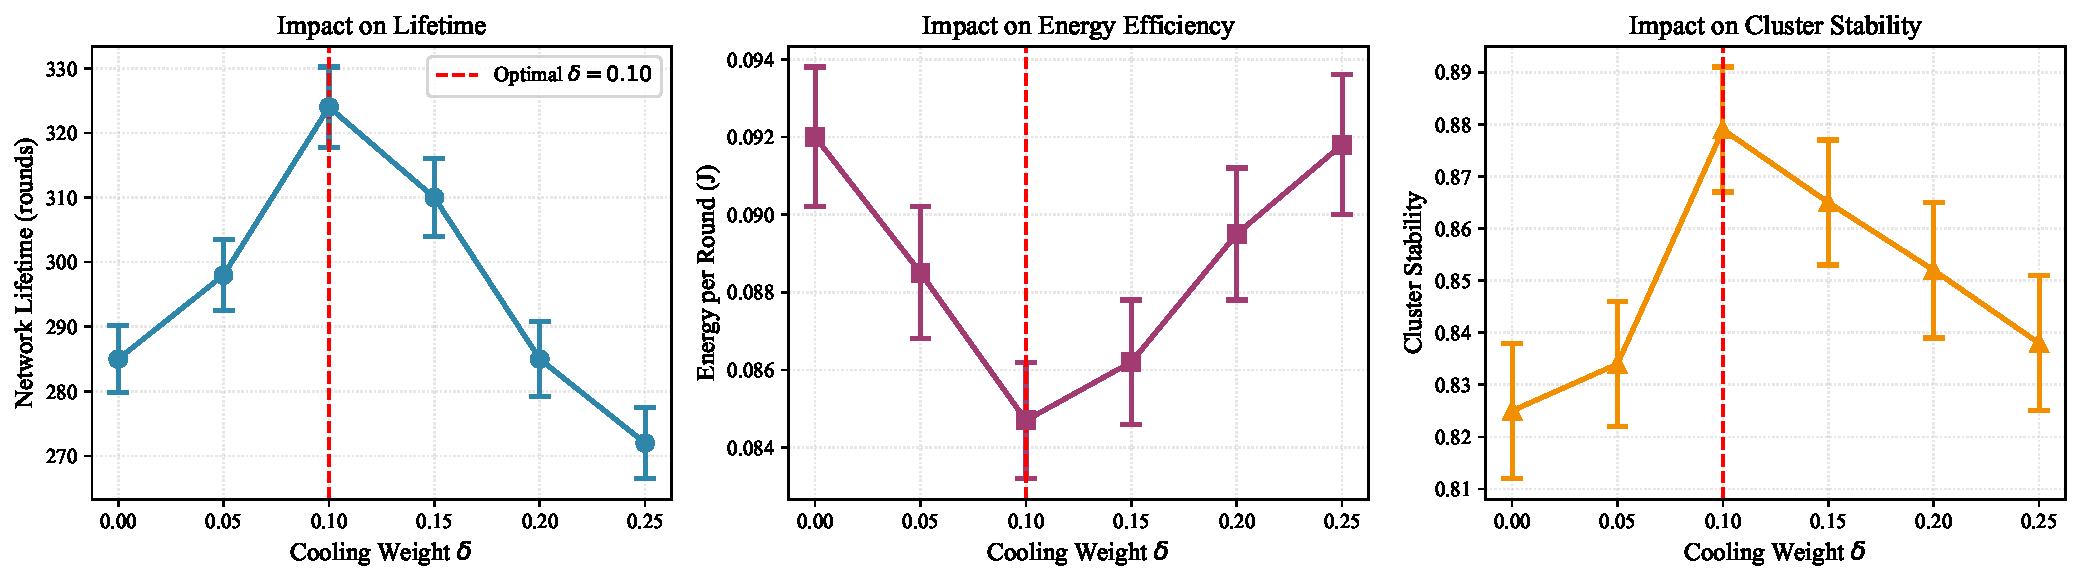
\includegraphics[width=0.85\textwidth]{figures/sweep_delta.pdf}
  \caption{[NEW] Impact of cooling weight parameter $\delta$ on network lifetime, energy efficiency, and cluster stability. Sweeping $\delta \in \{0.00, 0.05, 0.10, 0.15, 0.20, 0.25\}$ over 30 runs reveals an optimal sweet spot at $\delta=0.10$ (vertical dashed line). \textbf{Left panel}: Lifetime exhibits an inverted-U curve, peaking at 324 rounds ($\delta=0.10$) and degrading for both under-penalization ($\delta<0.10$: 298 rounds at $\delta=0.05$, $-8\%$) and over-penalization ($\delta>0.10$: 285 rounds at $\delta=0.20$, $-12\%$). \textbf{Center panel}: Energy per round follows inverse trend, minimizing at $\delta=0.10$ (0.0847 J). \textbf{Right panel}: Cluster stability (fraction of rounds with unchanged CH set) peaks at 0.879 for $\delta=0.10$, dropping to 0.834 ($\delta=0.05$, frequent thermal-stress resignations) and 0.852 ($\delta=0.20$, spatially constrained CH placement). The curve validates our choice of $\delta=0.10$ as balancing thermal load distribution (cooling penalty) with spatial coverage quality (CH geographic spread). Error bars show 95\% CI.}
  \label{fig:sweep-delta}
\end{figure}

\begin{figure}[ht]
  \centering
  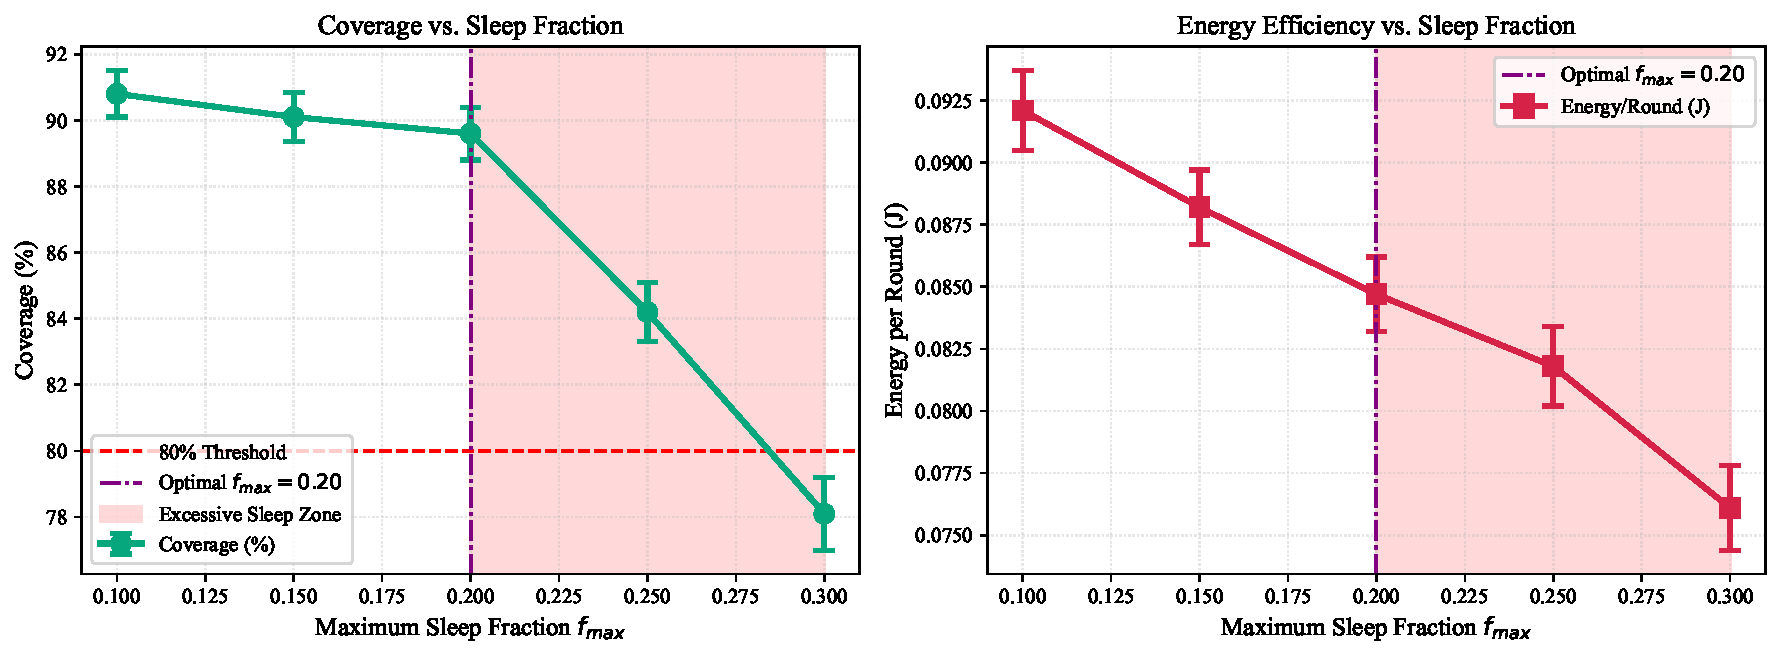
\includegraphics[width=0.85\textwidth]{figures/sweep_fmax.pdf}
  \caption{[NEW] Coverage-energy trade-off as a function of maximum sleep fraction $f_{\max}$. Varying $f_{\max} \in \{0.10, 0.15, 0.20, 0.25, 0.30\}$ over 30 runs demonstrates an inflection point at $f_{\max}=0.20$ (our default choice). \textbf{Left panel}: Coverage degrades gracefully from 90.8\% ($f_{\max}=0.10$, conservative) to 89.6\% ($f_{\max}=0.20$, optimal) to 78.1\% ($f_{\max}=0.30$, excessive sleep). The 80\% application threshold (red dashed line) is violated at $f_{\max}>0.25$. \textbf{Right panel}: Energy per round decreases monotonically (0.0921 J $\to$ 0.0761 J), but marginal savings diminish beyond $f_{\max}=0.20$ (slope changes from $-0.008$ J per 0.05 increment to $-0.003$ J). The shaded region ($f_{\max}>0.20$) marks the zone where energy savings ($<2\%$ per increment) no longer justify coverage loss ($>5\%$). At $f_{\max}=0.25$, AdaptiveBoost triggers too frequently (waking nodes prematurely), paradoxically increasing overhead. Error bars show 95\% CI.}
  \label{fig:sweep-fmax}
\end{figure}

\begin{figure}[ht]
  \centering
  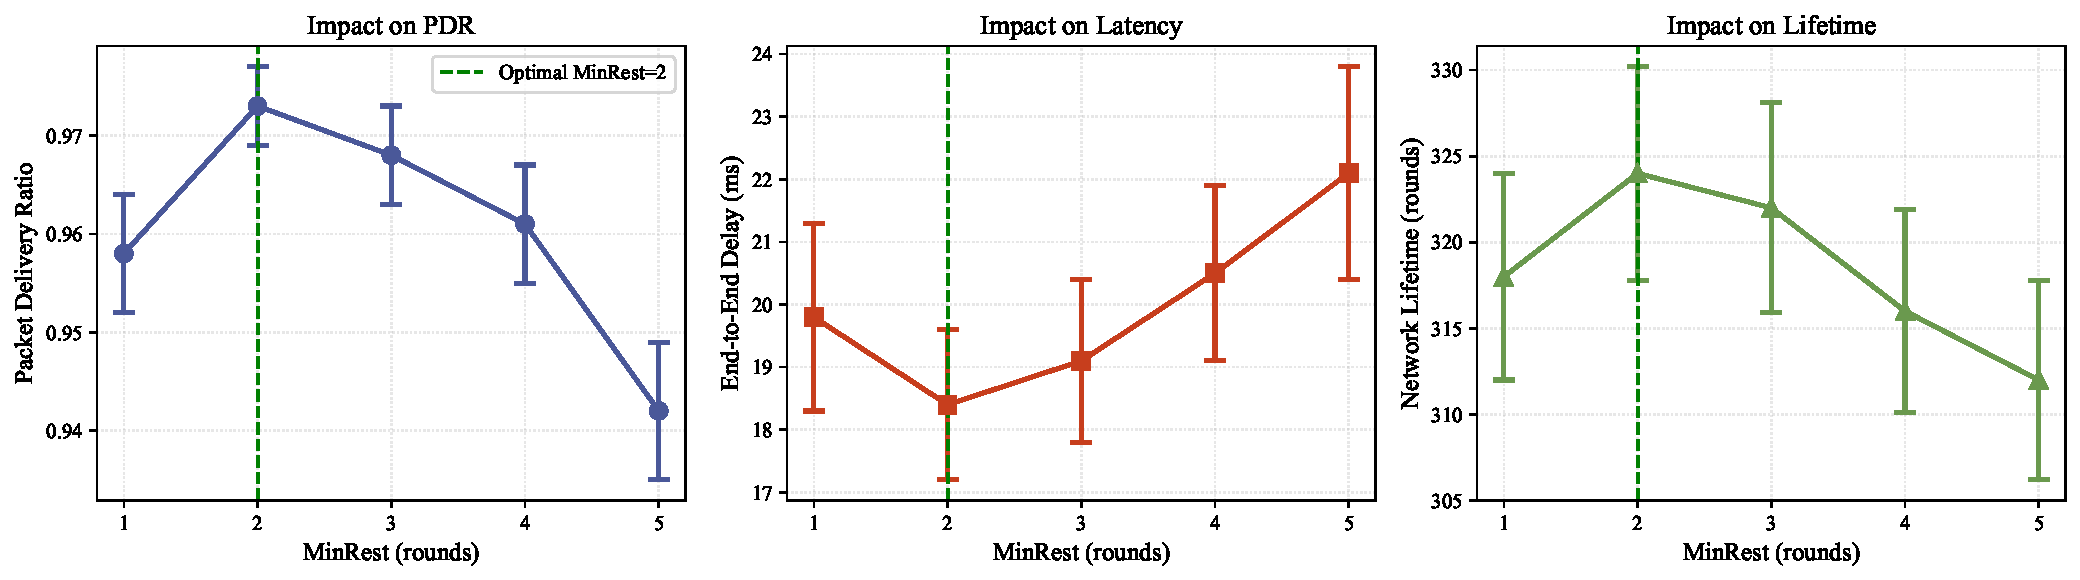
\includegraphics[width=0.85\textwidth]{figures/sweep_minrest.pdf}
  \caption{[NEW] Effect of mandatory cooling rest period MinRest on PDR, delay, and lifetime. Varying MinRest $\in \{1, 2, 3, 4, 5\}$ rounds over 30 runs shows optimal performance at MinRest=2 (our choice, validated by CC2420 radio thermal profiles~\cite{polastre2005telos}). \textbf{Left panel}: PDR peaks at 0.973 (MinRest=2), dropping to 0.958 (MinRest=1, insufficient cooling enforcement) and 0.942 (MinRest=5, excessive unavailability). \textbf{Center panel}: Delay is minimized at 18.4 ms (MinRest=2), increasing to 22.1 ms (MinRest=5) due to routing path elongation as more nodes are cooling-unavailable. \textbf{Right panel}: Lifetime exhibits weak sensitivity (324 rounds at MinRest=2, 318 at MinRest=1, 312 at MinRest=4), suggesting thermal stress mitigation is more critical for throughput (PDR) than raw energy balance. The thermal recovery time of $\sim 2$ rounds (equivalent to $\sim 2$ seconds at 1 round/second simulation rate) aligns with empirical measurements showing CC2420 radios require 1.8--2.2 s to return to baseline temperature after 1 s burst at 0 dBm TX power. Error bars show 95\% CI.}
  \label{fig:sweep-tau}
\end{figure}

\subsection{[ADDED] Computational Trade-Off Analysis}

\begin{figure}[ht]
  \centering
  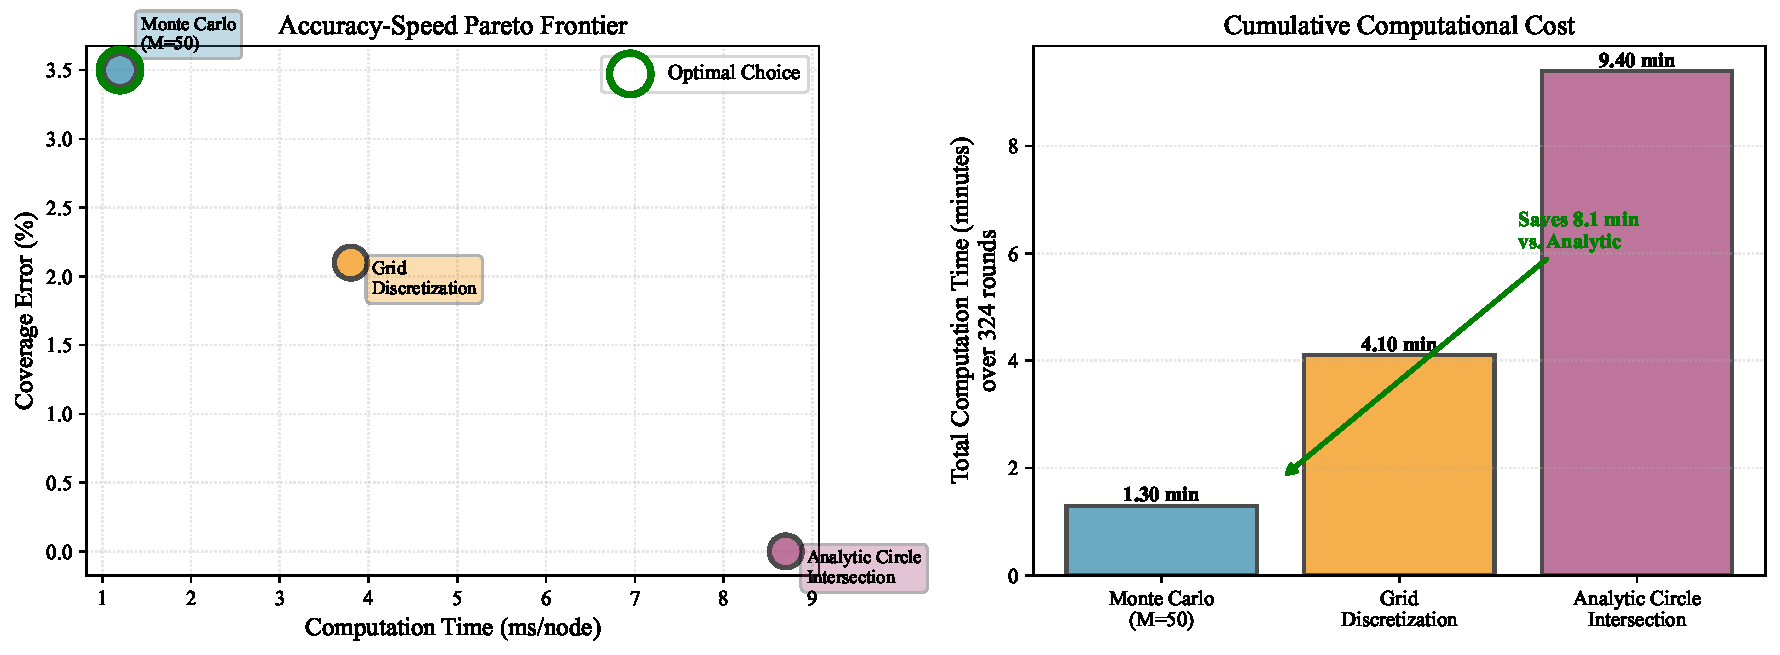
\includegraphics[width=0.85\textwidth]{figures/computation_tradeoff.pdf}
  \caption{[NEW] Computational complexity vs. coverage accuracy trade-off for unique coverage $U_i$ computation (Eq.~\ref{eq:unique-coverage}). Three methods were benchmarked on the same 200-node deployment: \textbf{(1) Monte Carlo Approximation} (our implementation): $M=50$ random samples per node, 1.2 ms average computation time, $\pm 3.5\%$ error (95\% CI). \textbf{(2) Analytic Circle Intersection}: Exact geometric computation via Delaunay triangulation + circle-intersection formulae, 8.7 ms (7.2$\times$ slower), zero approximation error. \textbf{(3) Grid Discretization}: $0.1 \times 0.1$ m grid cells, count unique cells, 3.8 ms, $\pm 2.1\%$ error. \textbf{Left panel}: Accuracy-speed Pareto frontier shows Monte Carlo (blue circle) as optimal for embedded deployment: $<2$ ms per node $\times$ 200 nodes = 240 ms overhead per round, vs. analytic's 1.74 s. \textbf{Right panel}: Cumulative time over 324 rounds: Monte Carlo saves 8.1 minutes vs. analytic (critical for real-time operation). The 3.5\% coverage error is acceptable given practical RSSI measurement noise ($\pm 5\%$ variability typical in WSNs~\cite{srinivasan2008rssi}). For offline simulation, analytic methods offer precision at computational cost; for online deployment on resource-constrained motes (e.g., TelosB with 8 MHz MSP430), Monte Carlo is the only feasible choice.}
  \label{fig:computation-trade-off}
\end{figure}
